\chapter{Моделирование и результаты} \label{results}

\section{Скорость сходимости к формации в зависимости от параметров модели}
Перед тем как приступить к основным экспериментам~--- изучению сходимости сходимости  модели в зависимости от свойств графа коммуникации~--- были изучены зависимости сходимости от основных параметров модели, чтобы основные эксперименты можно было провести в оптимальных условиях.

Ниже приведены графики некоторых зависимостей и сводная таблица \ref{tbl:model-params} с описанием того, как параметры модели влияют на скорость сходимости.

\begin{figure}[!h]
    \center{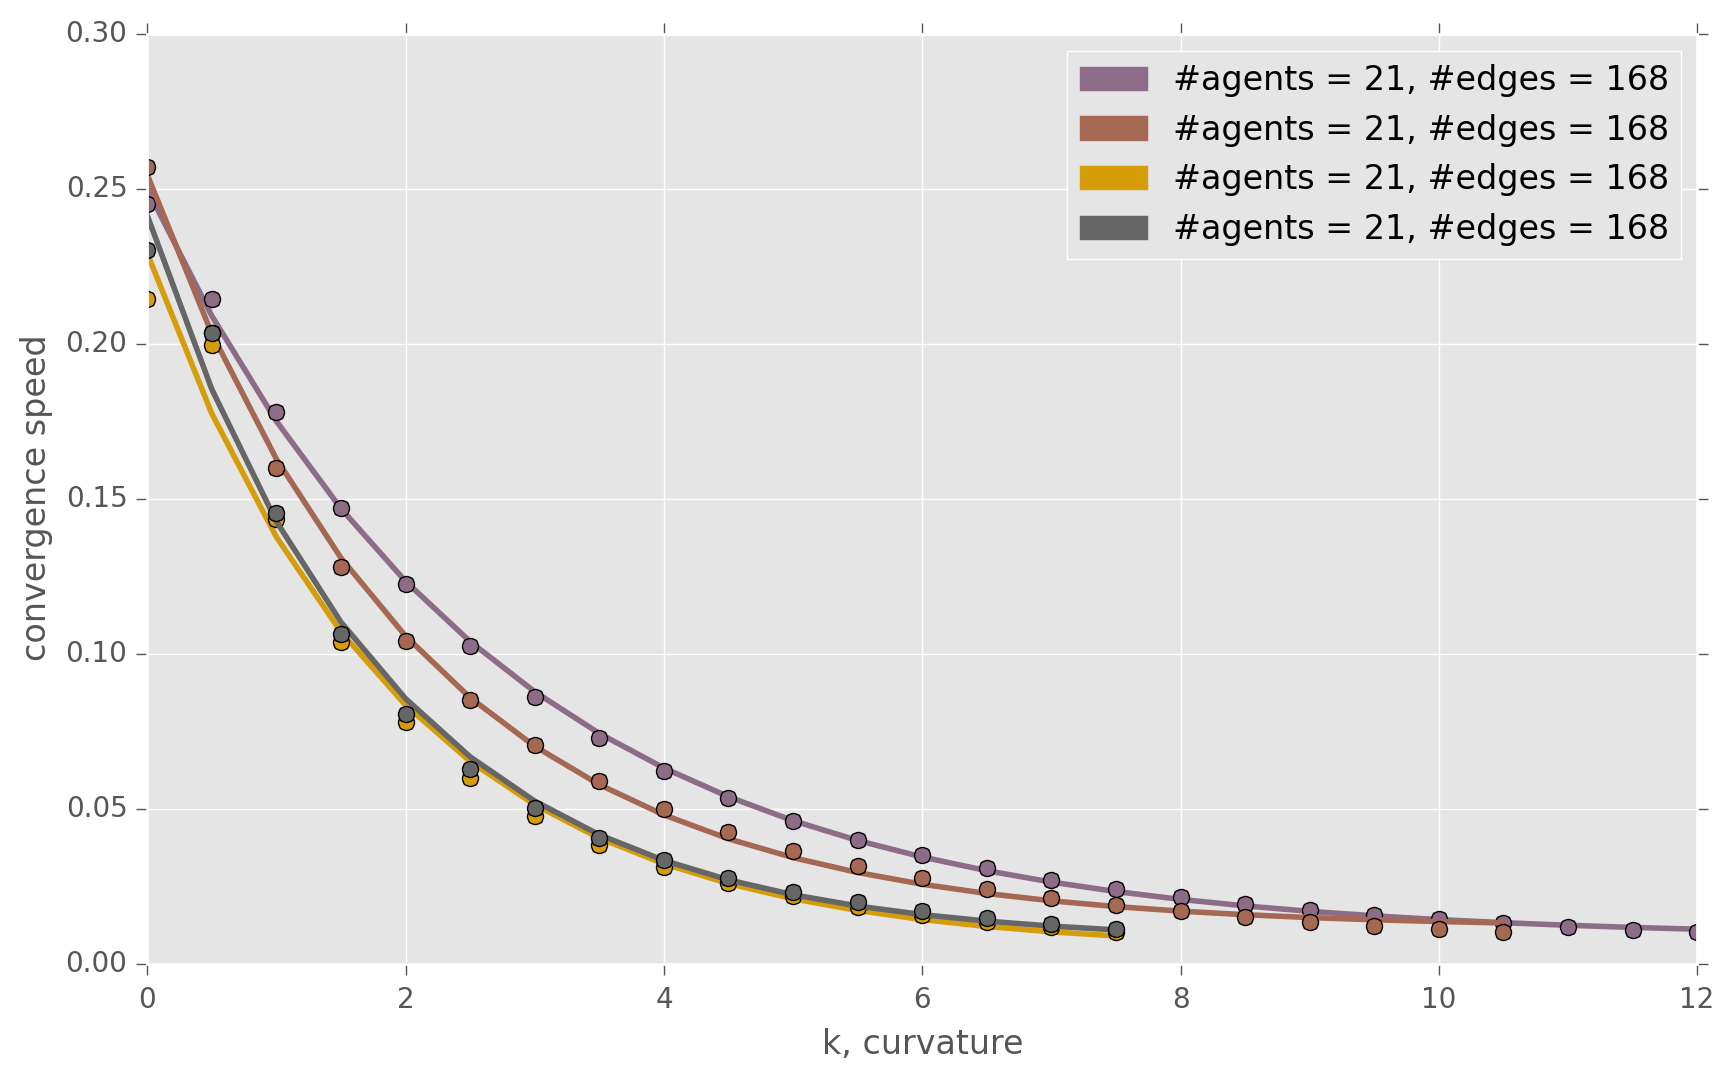
\includegraphics[width=0.9\linewidth, height=0.5\linewidth]{convergence_speed_curvature} 
  \caption{Скорость сходимости в зависимости от кривизны траектории $k$ для нескольких  случайных графов влияний. Во всех случаях число агентов $N=21$, количество ребер $168$, меняется начальная конфигурация и желаемая формация.}
  \label{img:convergence-k}  
\end{figure}

\begin{figure}[!h]
    \center{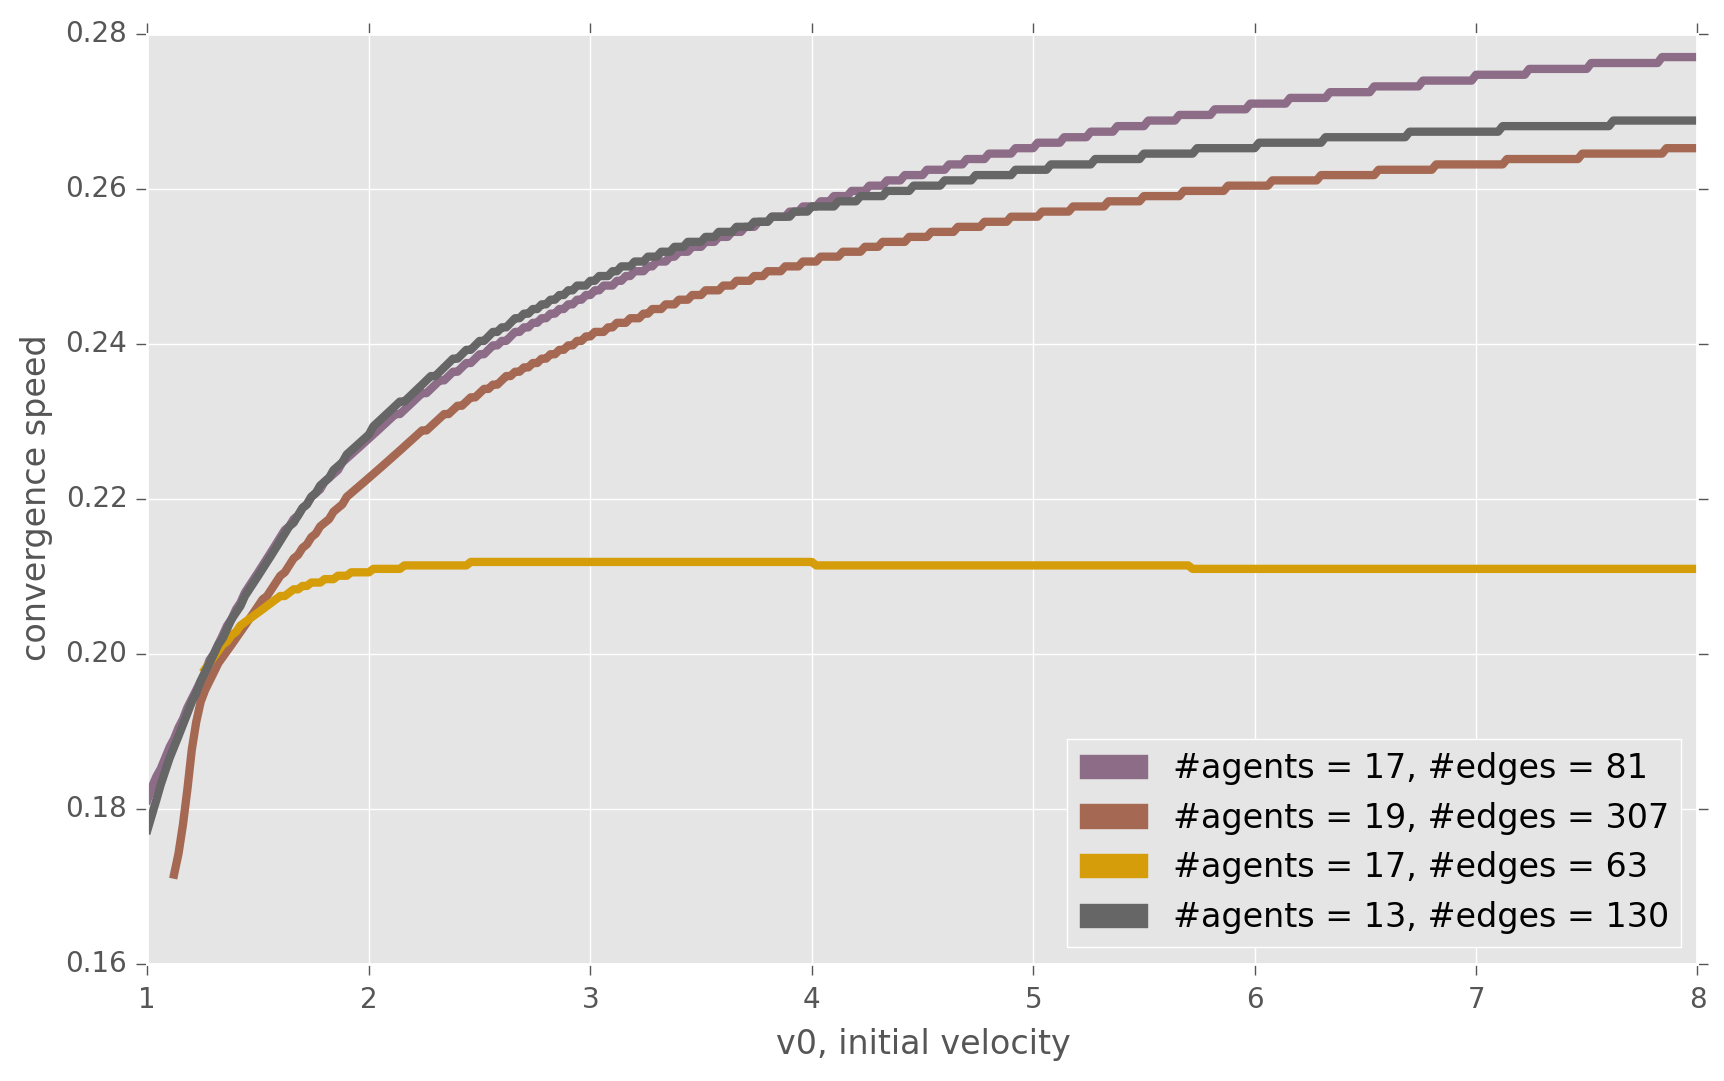
\includegraphics[width=0.9\linewidth, height=0.5\linewidth]{convergence_speed_v0} 
  \caption{Скорость сходимости в зависимости от начальной скорости агентов $v_0$. для нескольких  случайных графов влияний. Измерения при меньших скоростях затруднены, т.к. модель плохо сходится при малых скоростях.}
  \label{img:convergence-v0}  
\end{figure}

\begin{figure}[!h]
    \center{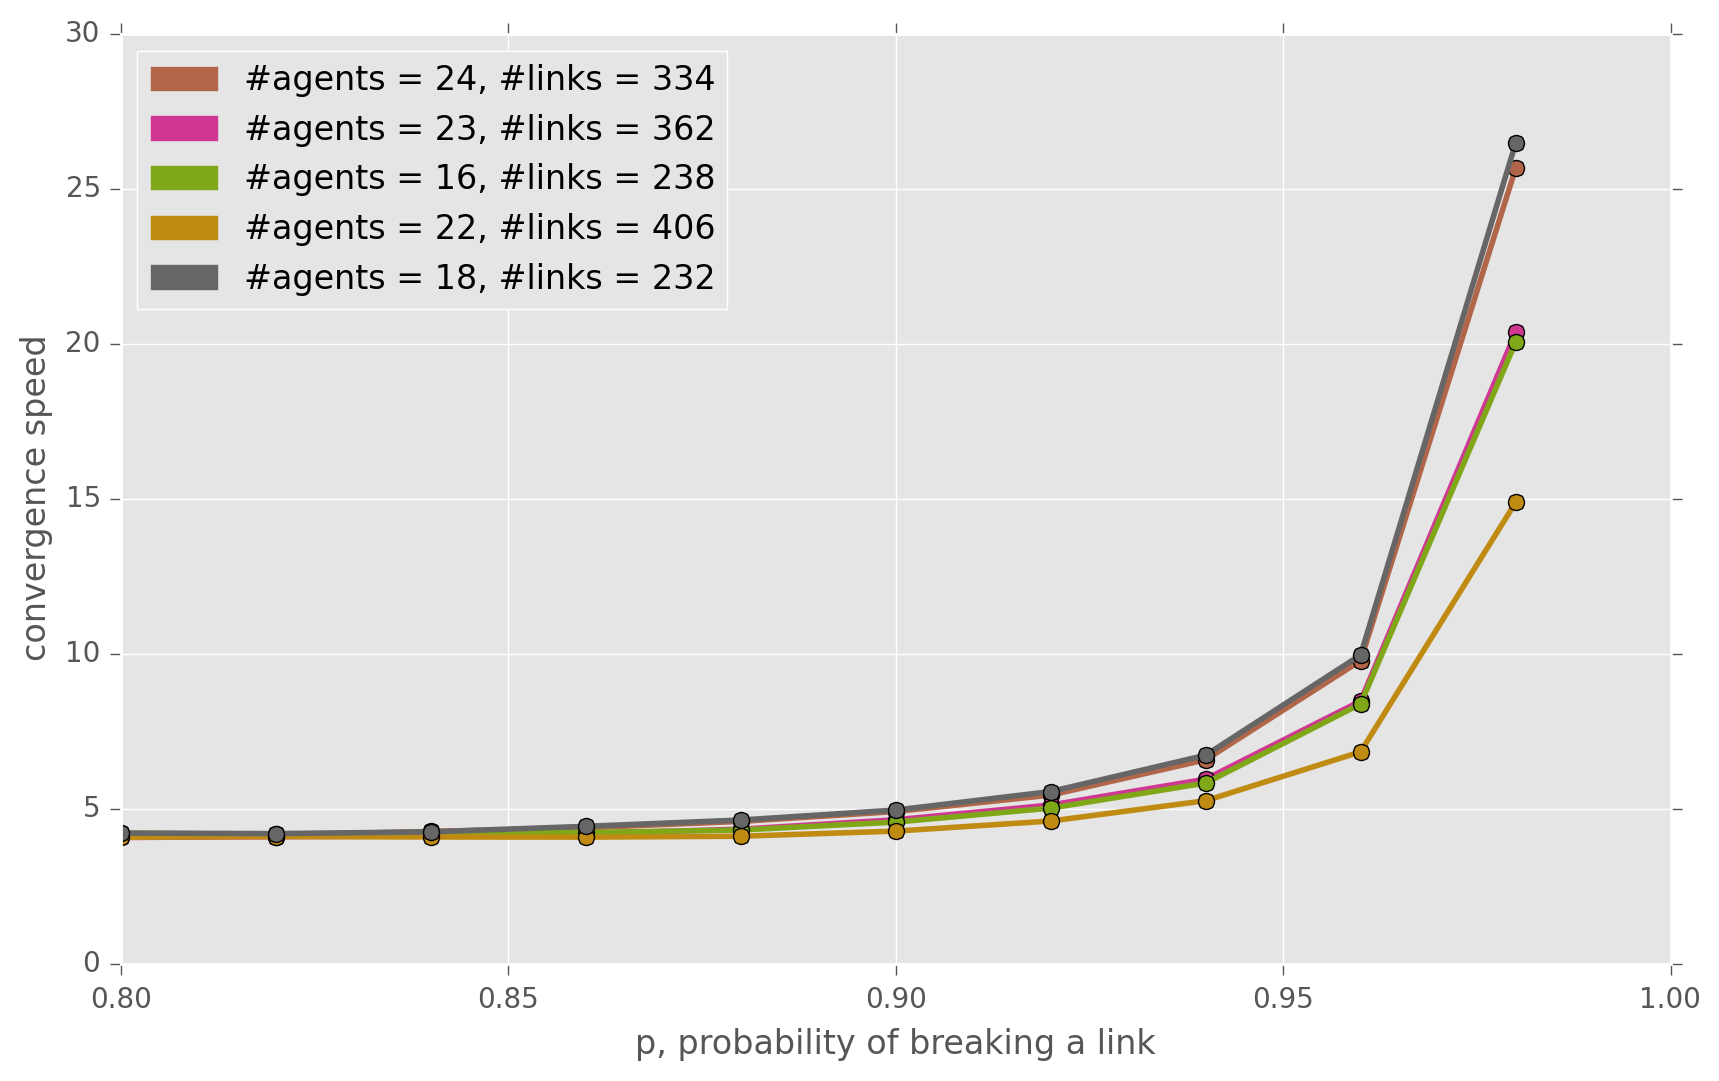
\includegraphics[width=0.9\linewidth, height=0.5\linewidth]{convergence_speed_p} 
  \caption{Скорость сходимости в зависимости от параметра $p$, вероятности разрыва связи на каждом шаге симуляции для разных чисел агентов и графов влияний. Для каждого графа показан результат усреднения по 50 экспериментам для каждого значения $p$.}
   \label{img:graphs-convergence-p}  
\end{figure}

\begin{table} [!htbp]
  \centering
  \parbox{15cm}{\caption{Скорость сходимости в зависимости от параметров модели}\label{tbl:model-params}}
\begin{tabular}{| L{7cm} | L{7cm} |}
\hline
\textbf{Параметр} & \textbf{Влияние на скорость сходимости} \\
\hline
$p$, вероятность разрыва ребра & $\sim A+B\exp(C(p-p_0))$ \\
\hline
$k$, кривизна траектории & $\sim A+B\exp(-C p)$ \\
\hline
$v_0$, величина начальной скорости & Замедляющийся рост и последующий выход на константный уровень \\
\hline
$D$, интенсивность расталкивания & В отдельных случаях может как ускорить, так и замедлить сходимость. В работе подробно не исследовалось \\
\hline
$f_1,\ f_2$, коэффициенты обратной связи. & В данной работе не изучено, но в  \cite{lafferriere2005decentralized} говорится, что при возрастании модулей $f_{1,2}$ увеличивается скорость сходимости. \\
\hline
\end{tabular}
\end{table}


\section{Скорость сходимости в зависимости от числа ребер графа коммуникации}
В работе изучена связь между числом ребер графа и скоростью сходимости к формации. При этом, чтобы учитывать только количество ребер, но не детали структуры графа, изучаются случайные графы, единственным ограничением для которых является наличие остовного исходящего дерева (необходимое условие сходимости модели). 

Общий вид зависимости одинаков для разных начальных параметров модели:
\begin{figure}[!h]
    \center{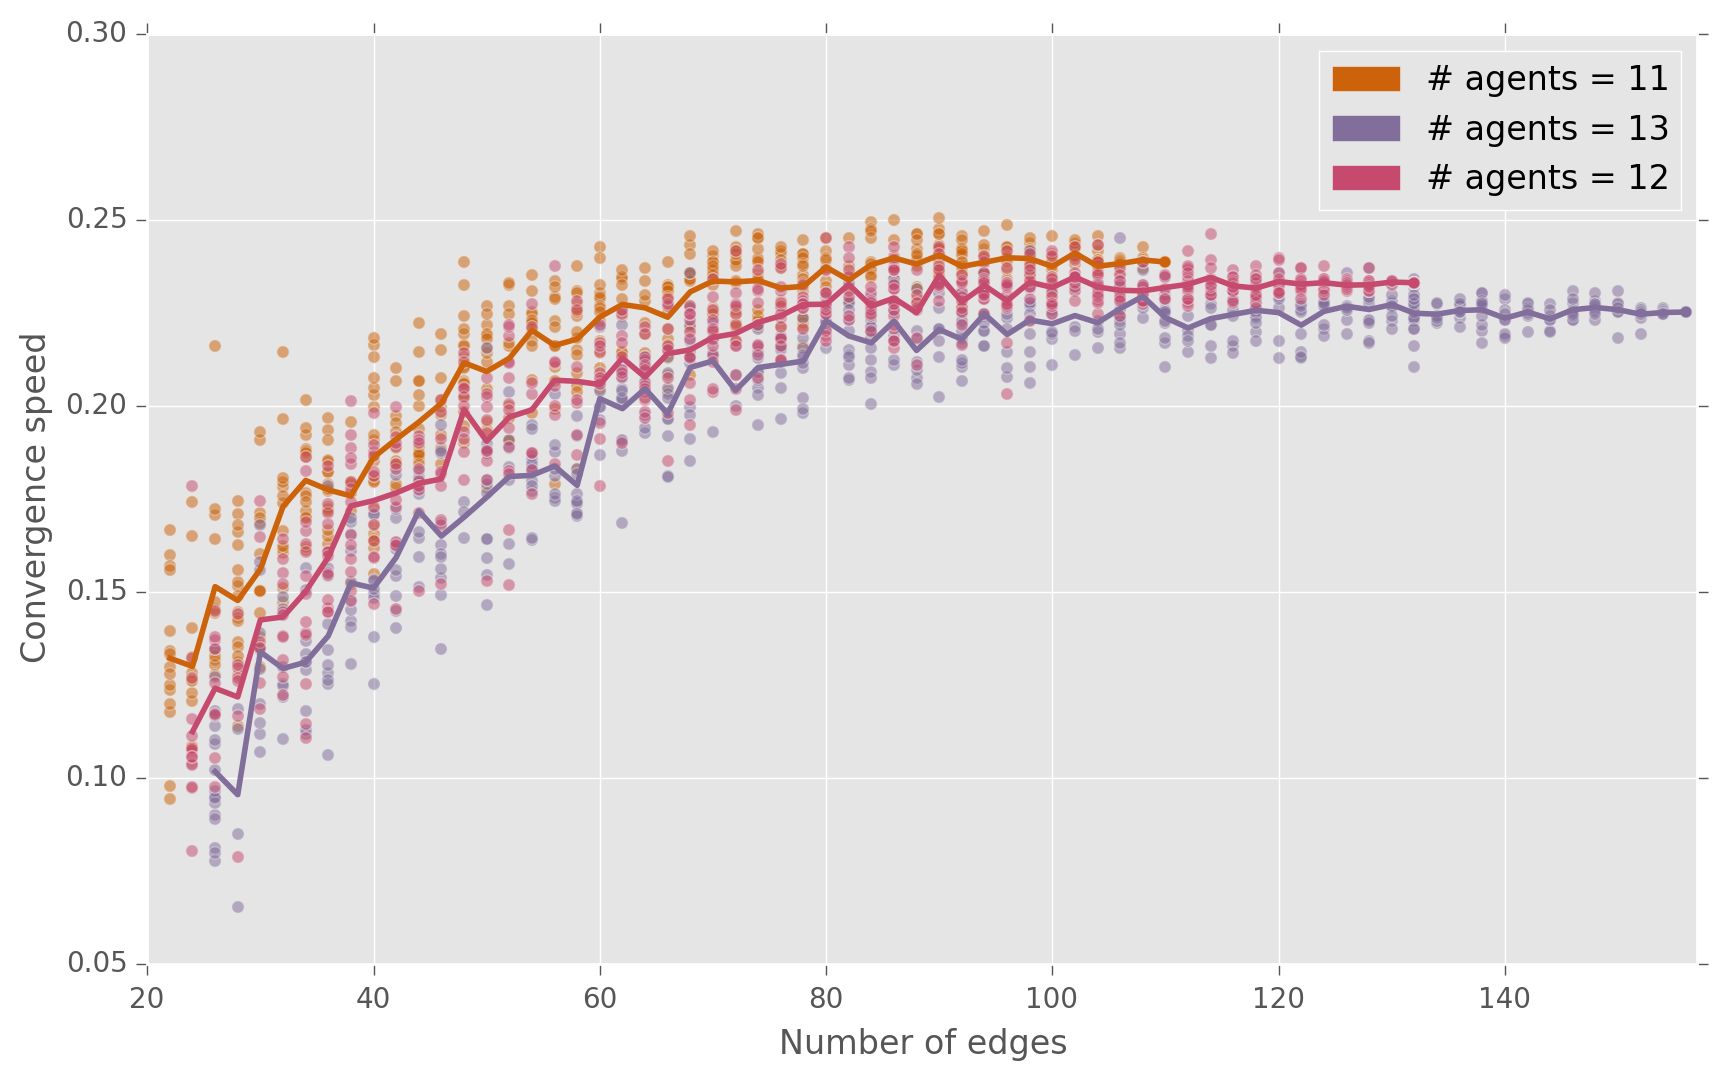
\includegraphics[width=0.9\linewidth]{convergence_speed_number_of_edges} 
  \caption{Скорость сходимости в зависимости от числа ребер для случаев $N=11,\ 12,\ 13.$ Линией выделены средние значения по 15 экспериментам для каждого значения числа ребер. Скачки вызваны небольшим числом экспериментов.}
  \label{img:graphs-edges}  
\end{figure}

В каждом из трех случаев параметры модели оставались одинаковыми, но менялись графы коммуникации. Использовались случайные графы с заданным числом ребер.

Так как скорость сходимости демонстрирует монотонный рост по мере увеличения числа ребер, имеет смысл задача максимизации скорости сходимости при заданном фиксированном числе ребер. Это ограничение имеет практический смысл при построении реальных систем.

\section{Скорость сходимости для графов разной структуры при фиксированном количестве ребер}

При фиксированном числе ребер графа влияний в модели имеет место положительная корреляция скорости сходимости и алгебраической связности графа. Поэтому для большей наглядности результаты экспериментов представлены в осях "скорость сходимости"--"алгебраическая связность".

В работе изучены следующие два предельных случая: 
\begin{itemize}
\item Графы, максимально однородные по степеням вершин и
\item Графы, максимально неоднородные по степеням вершин.
\end{itemize}

Примеры графов первой группы:

\begin{figure}[!h]
  \begin{minipage}[h]{0.29\linewidth}
    \center{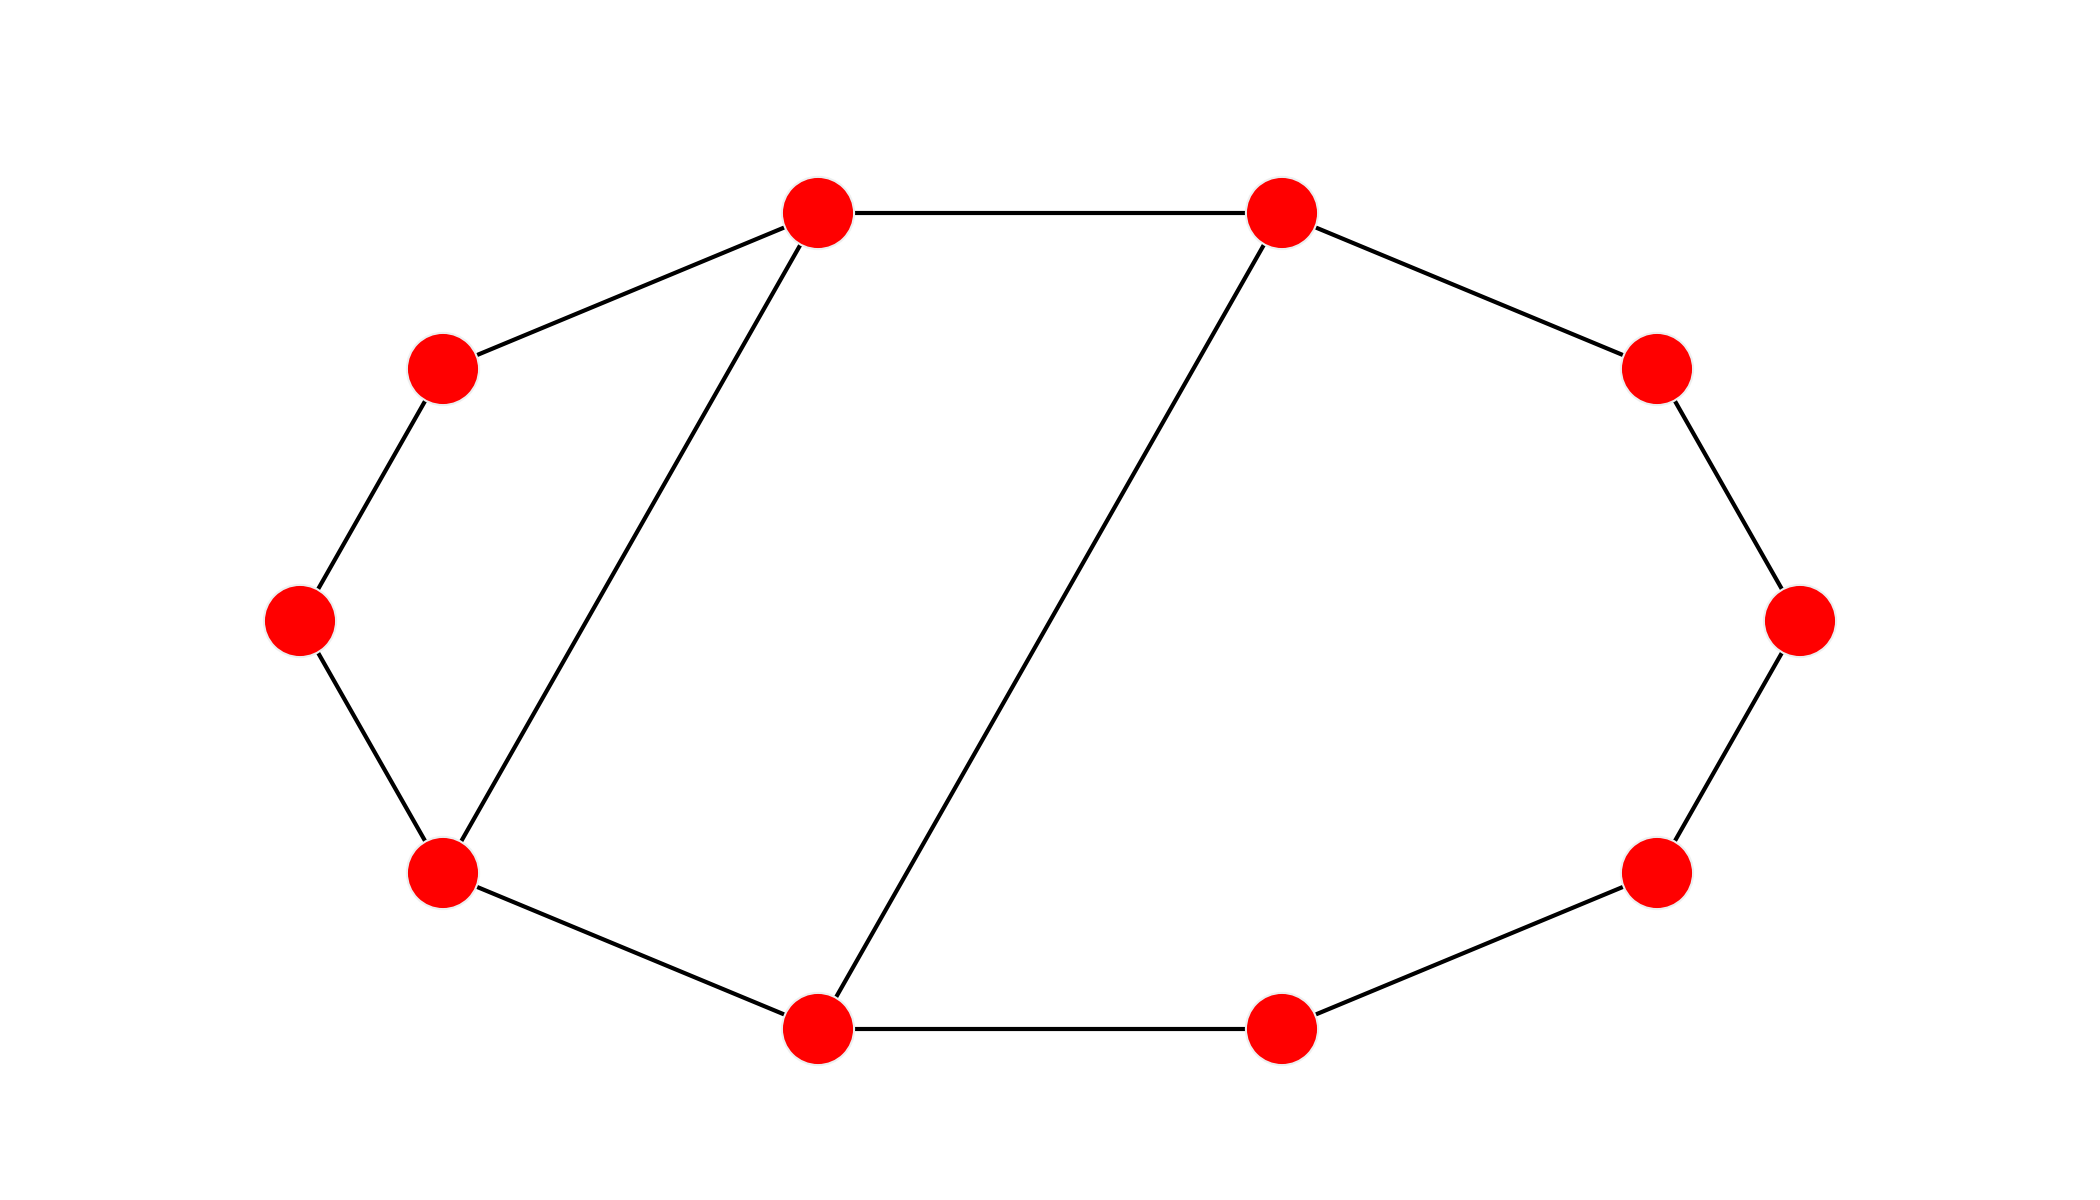
\includegraphics[width=1.2\linewidth]{graph_uniform_10_12} \\ а)}
  \end{minipage}
  \hfill
  \begin{minipage}[h]{0.29\linewidth}
    \center{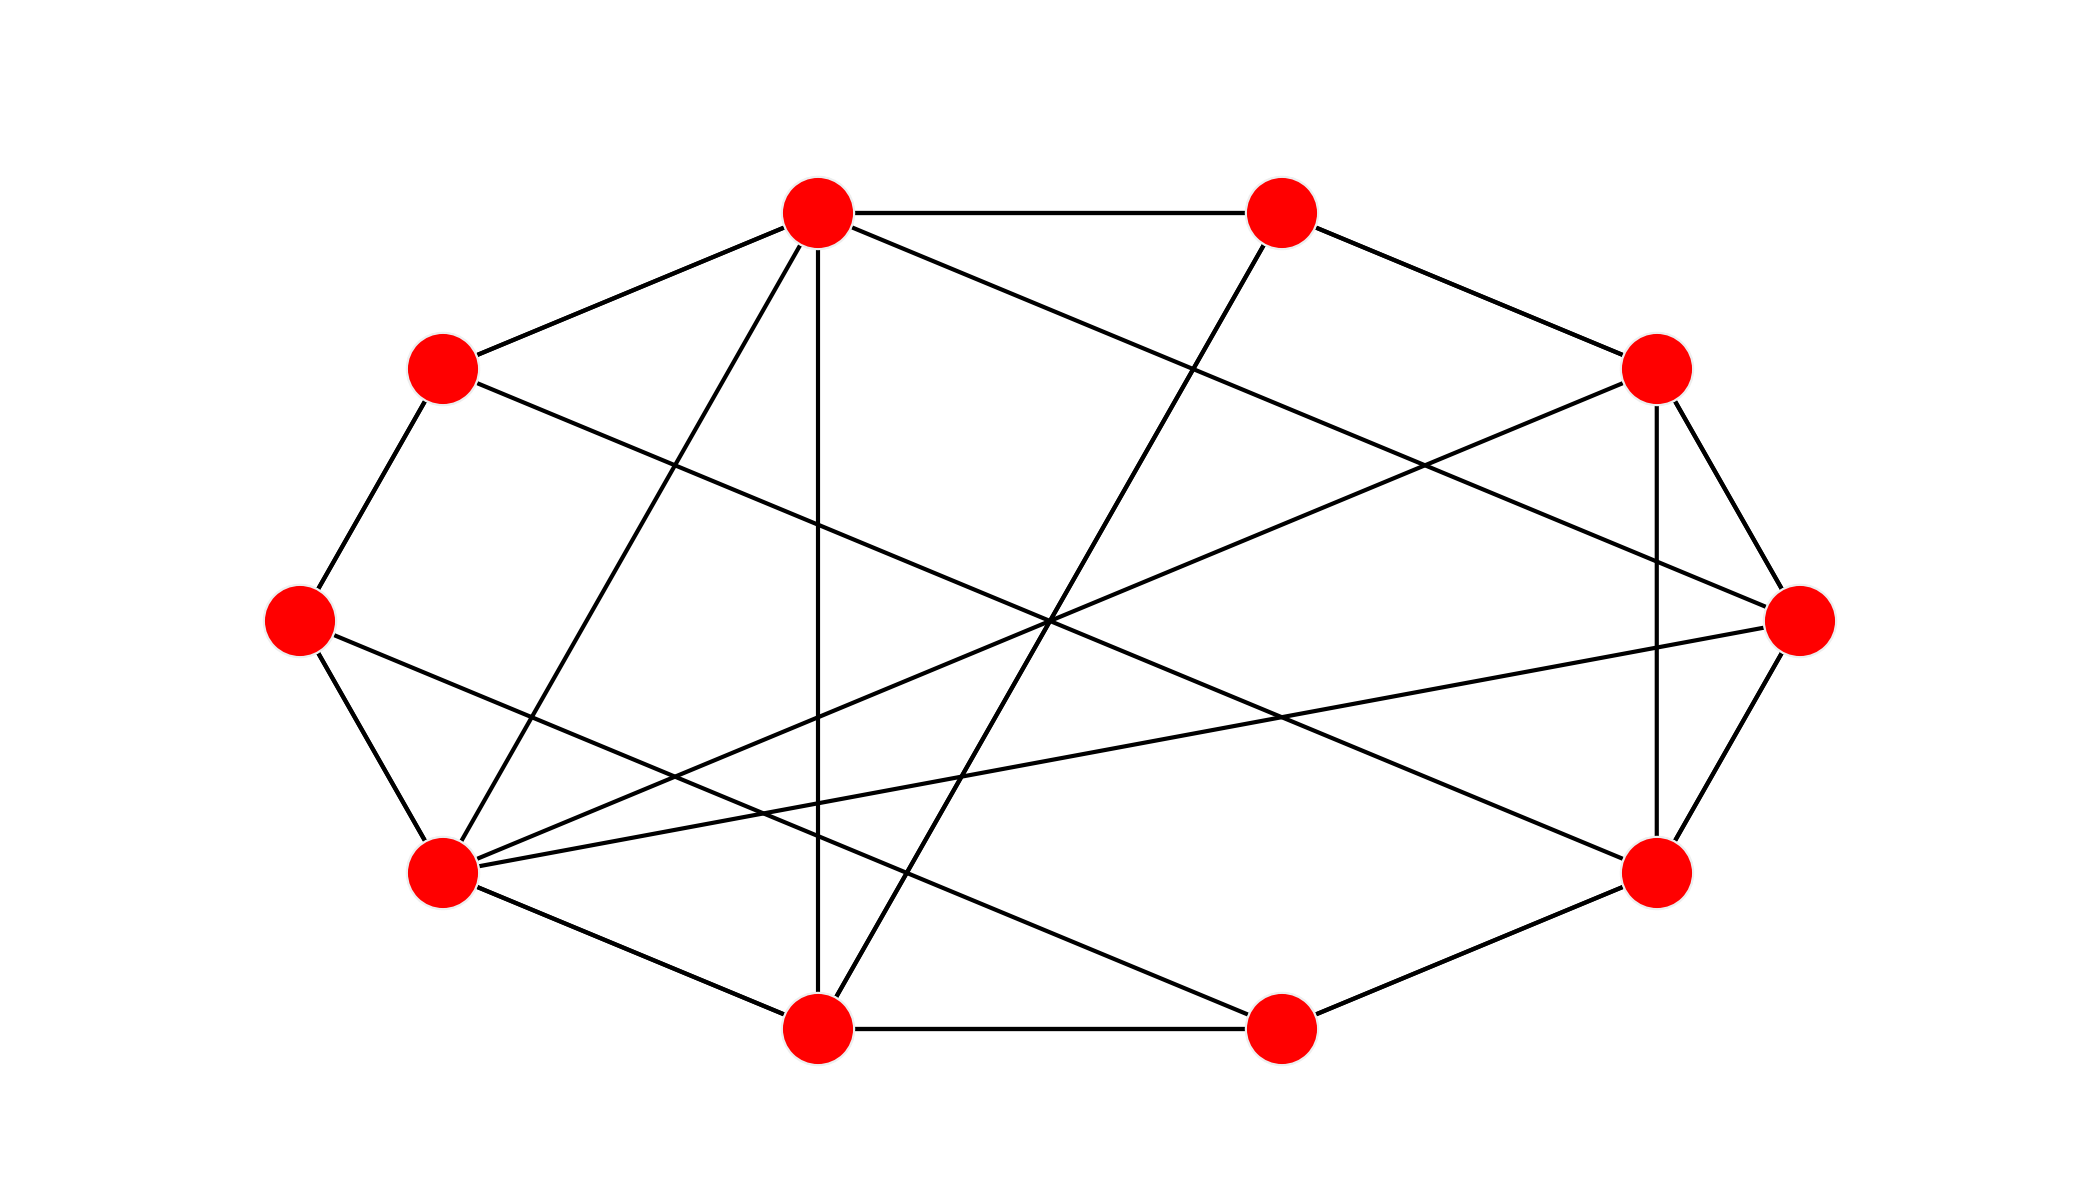
\includegraphics[width=1.2\linewidth]{graph_uniform_10_18} \\ б)}
  \end{minipage}
  \hfill
  \begin{minipage}[h]{0.29\linewidth}
    \center{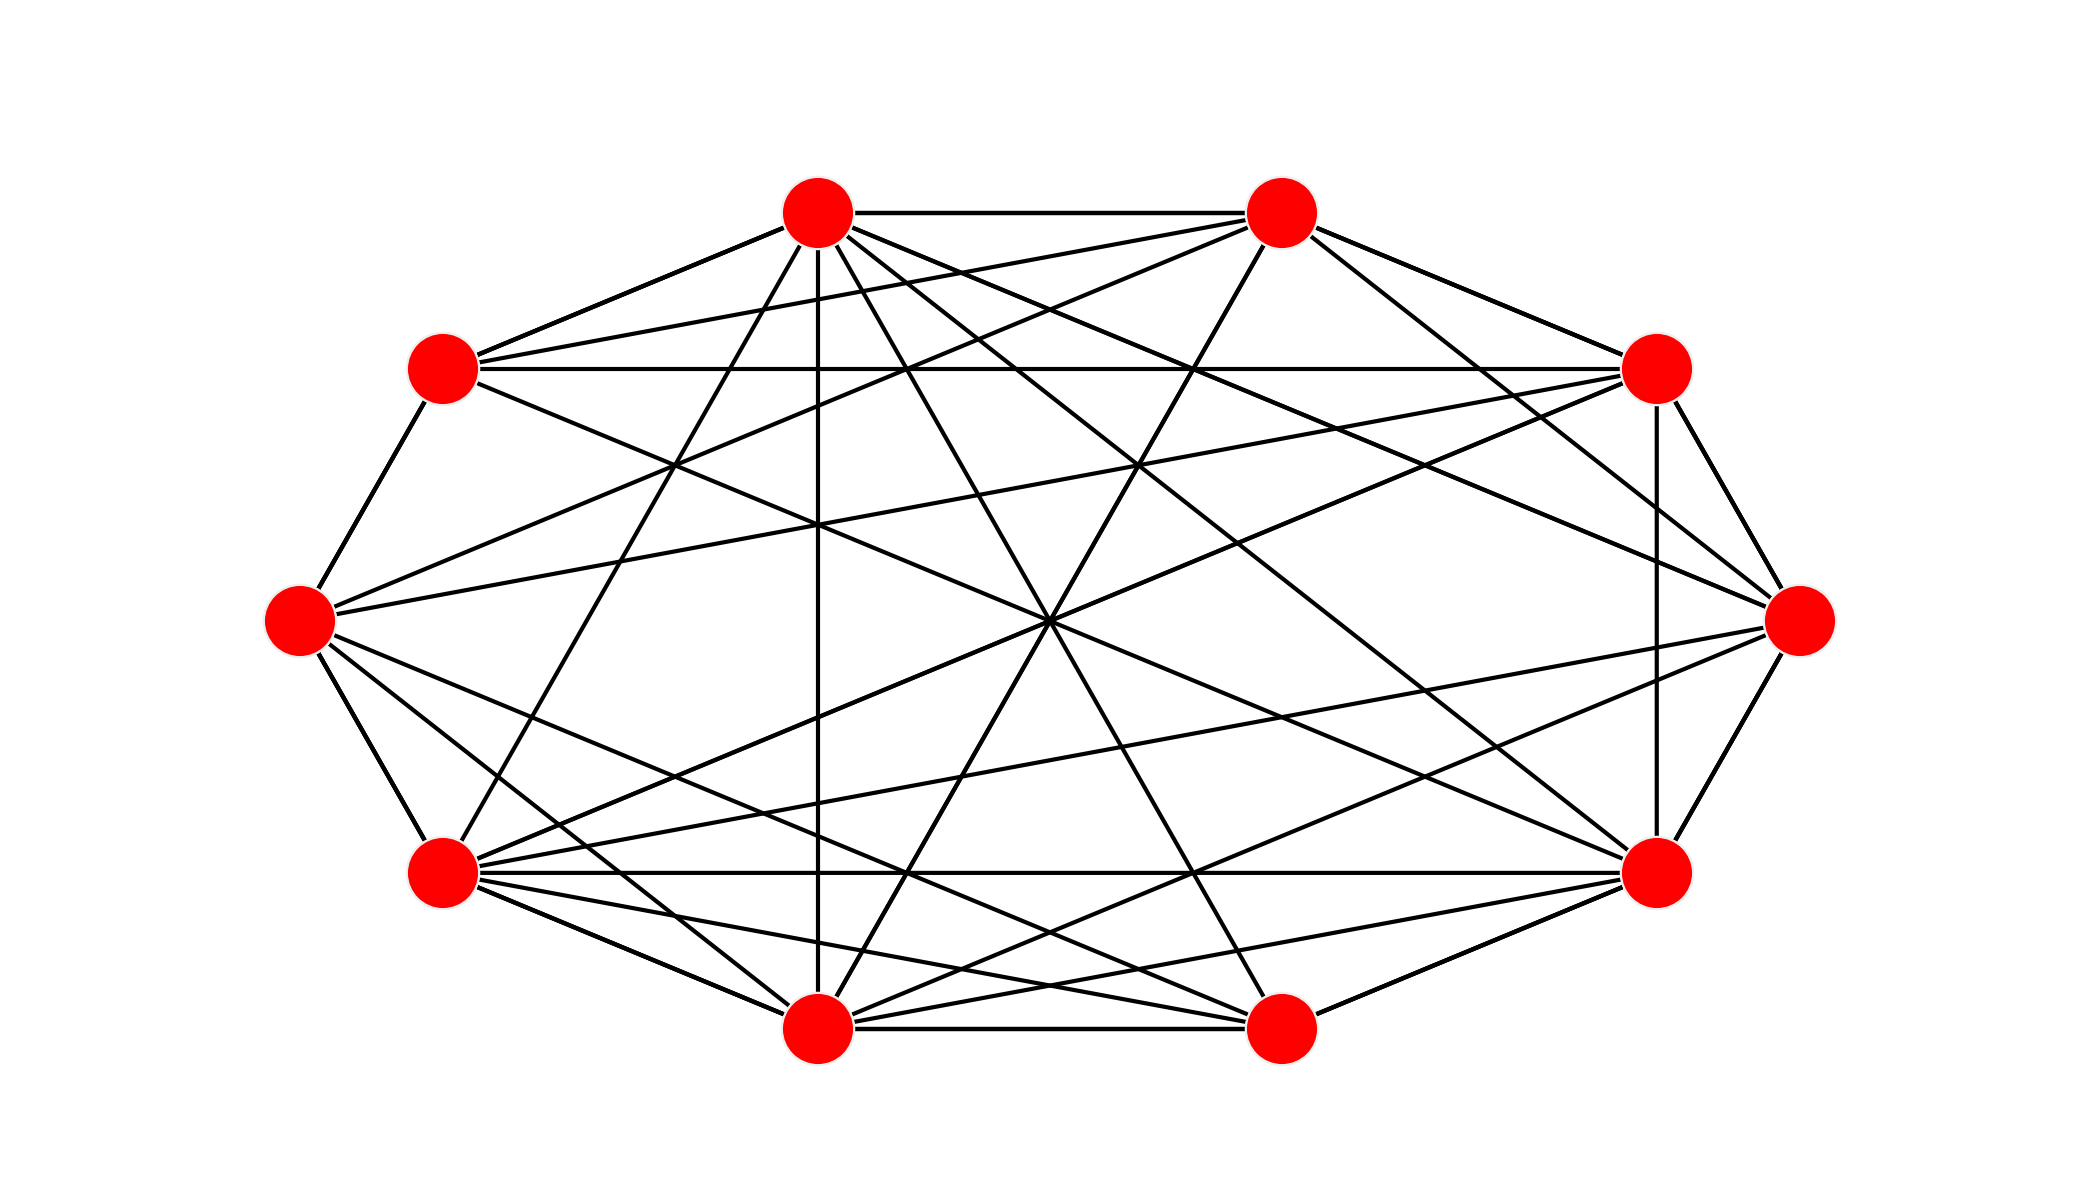
\includegraphics[width=1.2\linewidth]{graph_uniform_10_24} \\ в)}
  \end{minipage}
  \caption{Примеры графов, однородных по степеням вершин. \\ Количество вершин: 10, Слева направо: 12, 18, 24 ребра.}
  \label{img:graphs-uniform}  
\end{figure}

Графы второй группы были зашумлены добавлением случайных ребер для того, чтобы получить б\emph{о}льший диапазон алгебраической связности. \footnote{В отсутствии шума алгебраическая связность подобных графов часто равна целым числам.}

Примеры графов второй группы:

\begin{figure}[!h]
  \begin{minipage}[h]{0.29\linewidth}
    \center{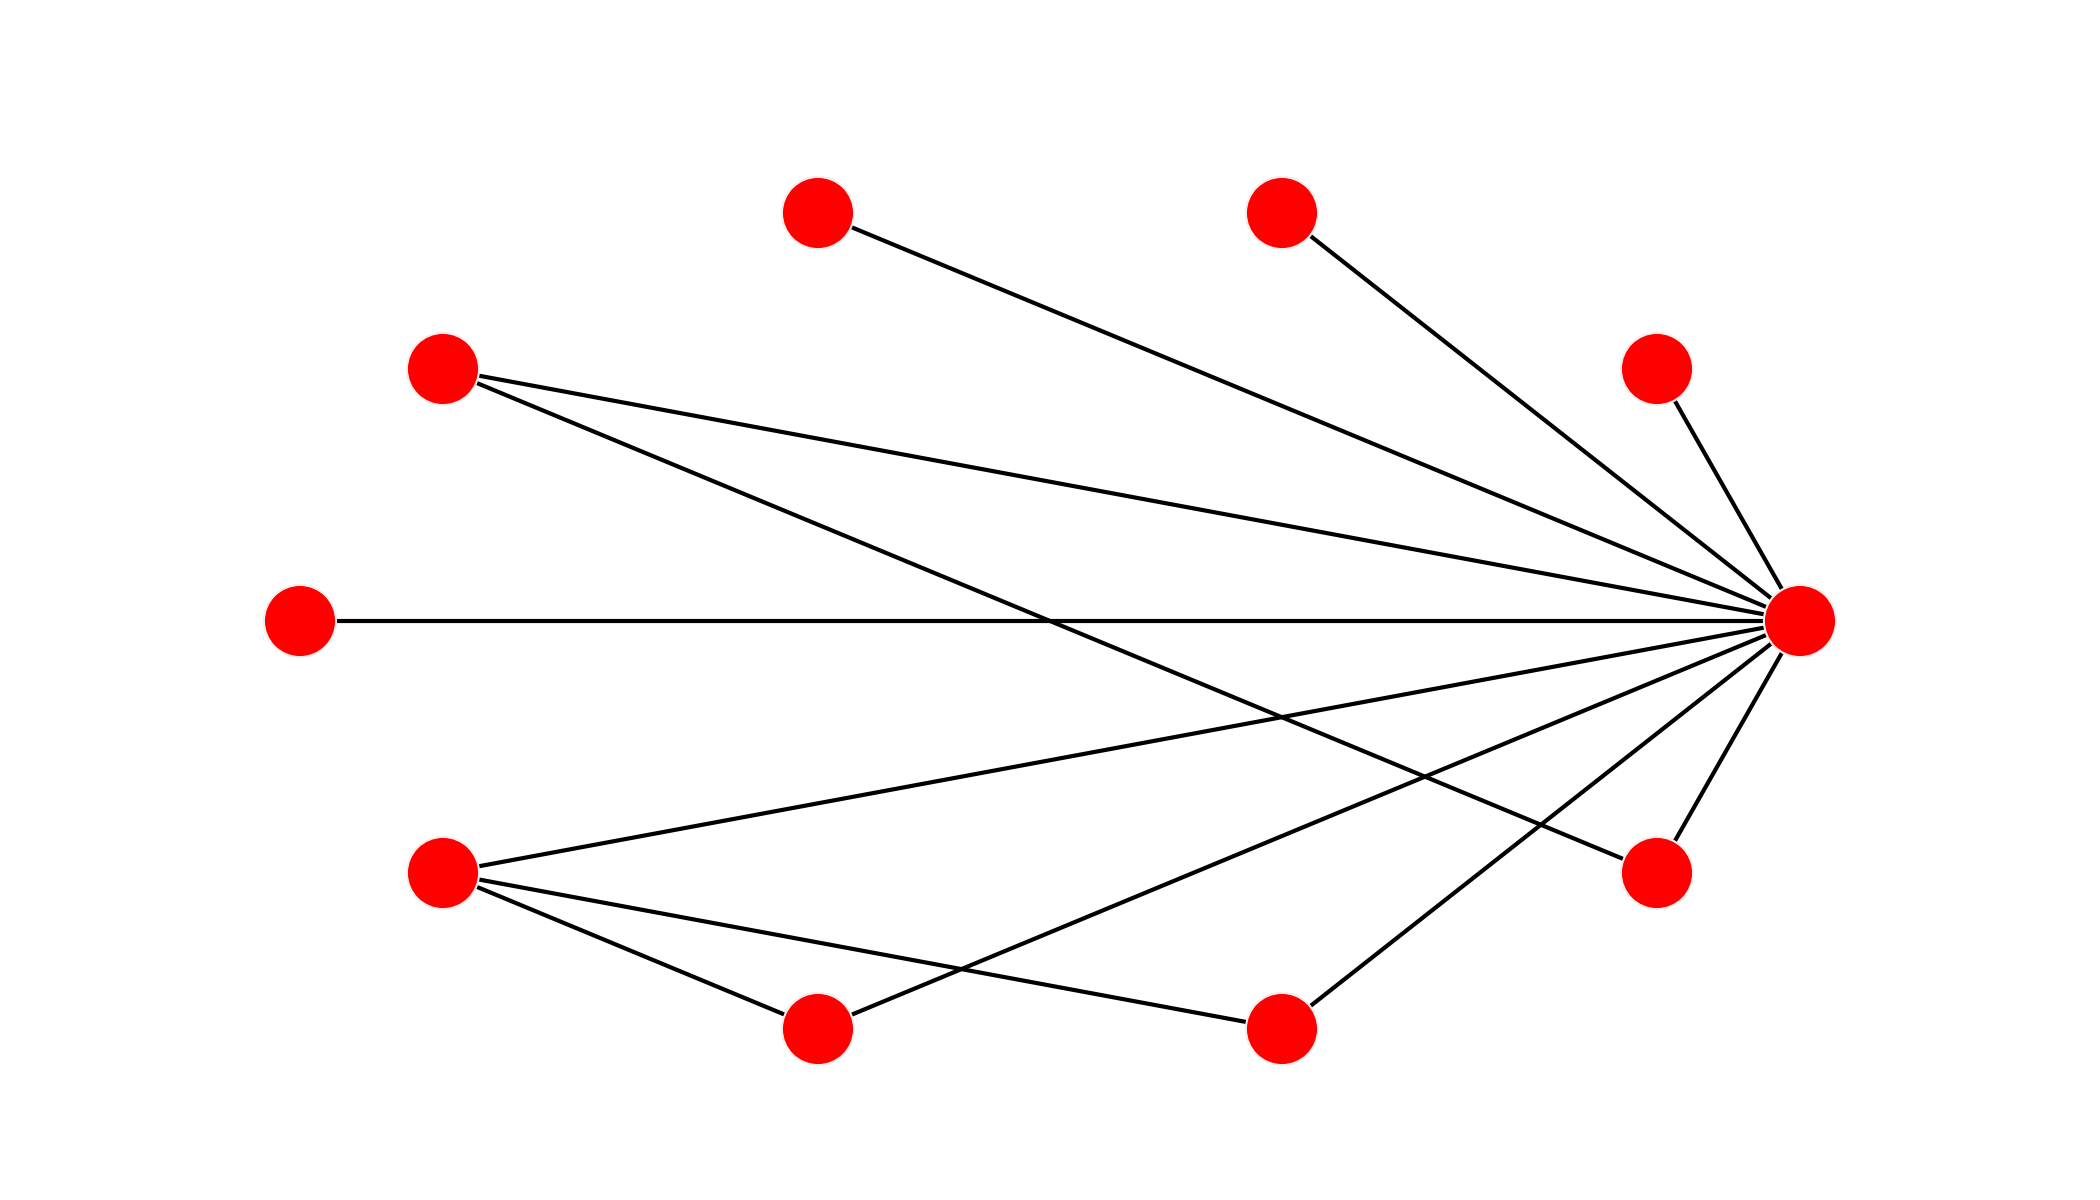
\includegraphics[width=1.2\linewidth]{graph_nonuniform_10_12} \\ а)}
  \end{minipage}
  \hfill
  \begin{minipage}[h]{0.29\linewidth}
    \center{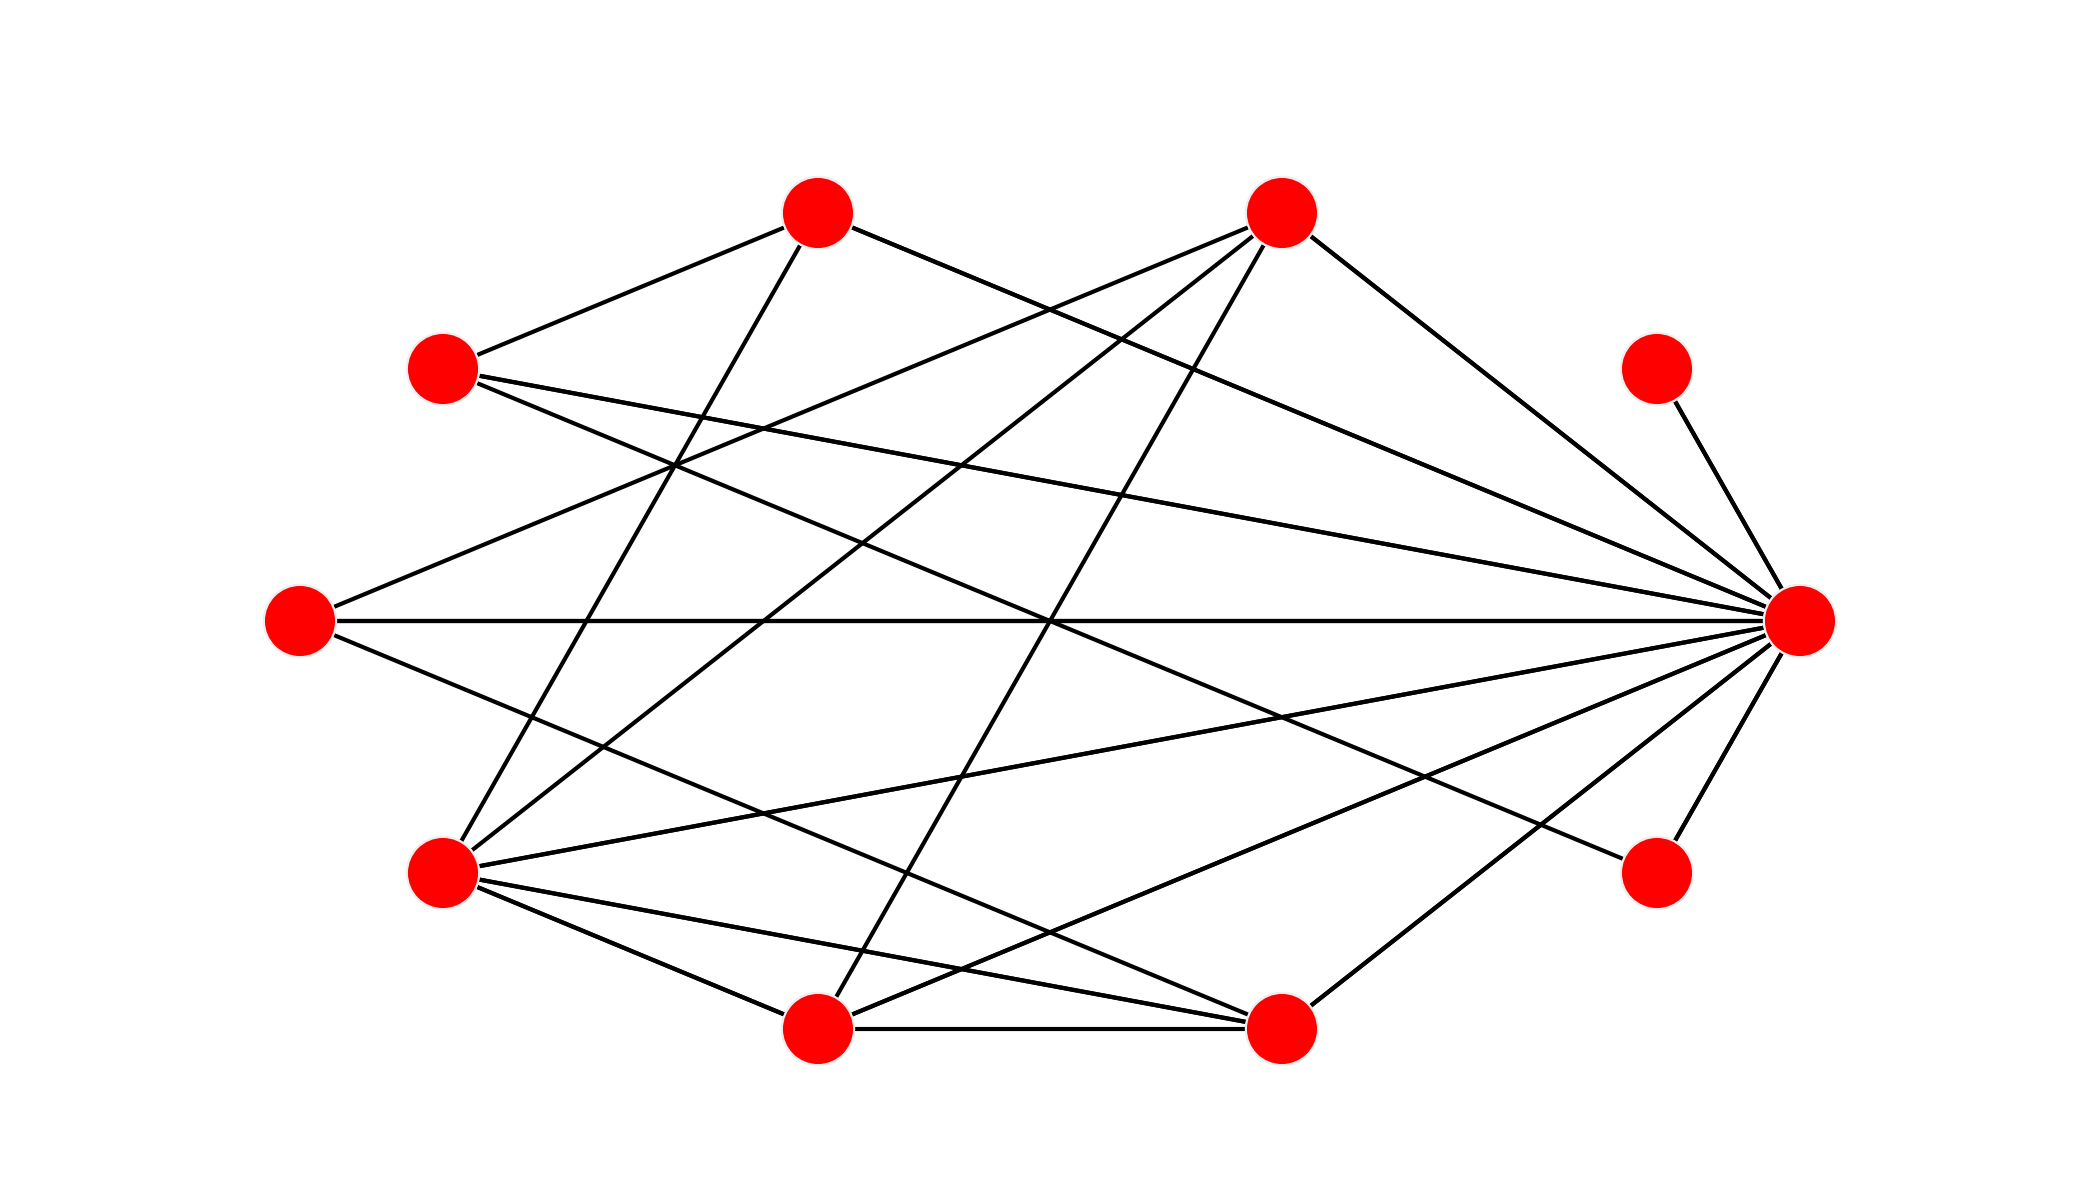
\includegraphics[width=1.2\linewidth]{graph_nonuniform_10_18} \\ б)}
  \end{minipage}
  \hfill
  \begin{minipage}[h]{0.29\linewidth}
    \center{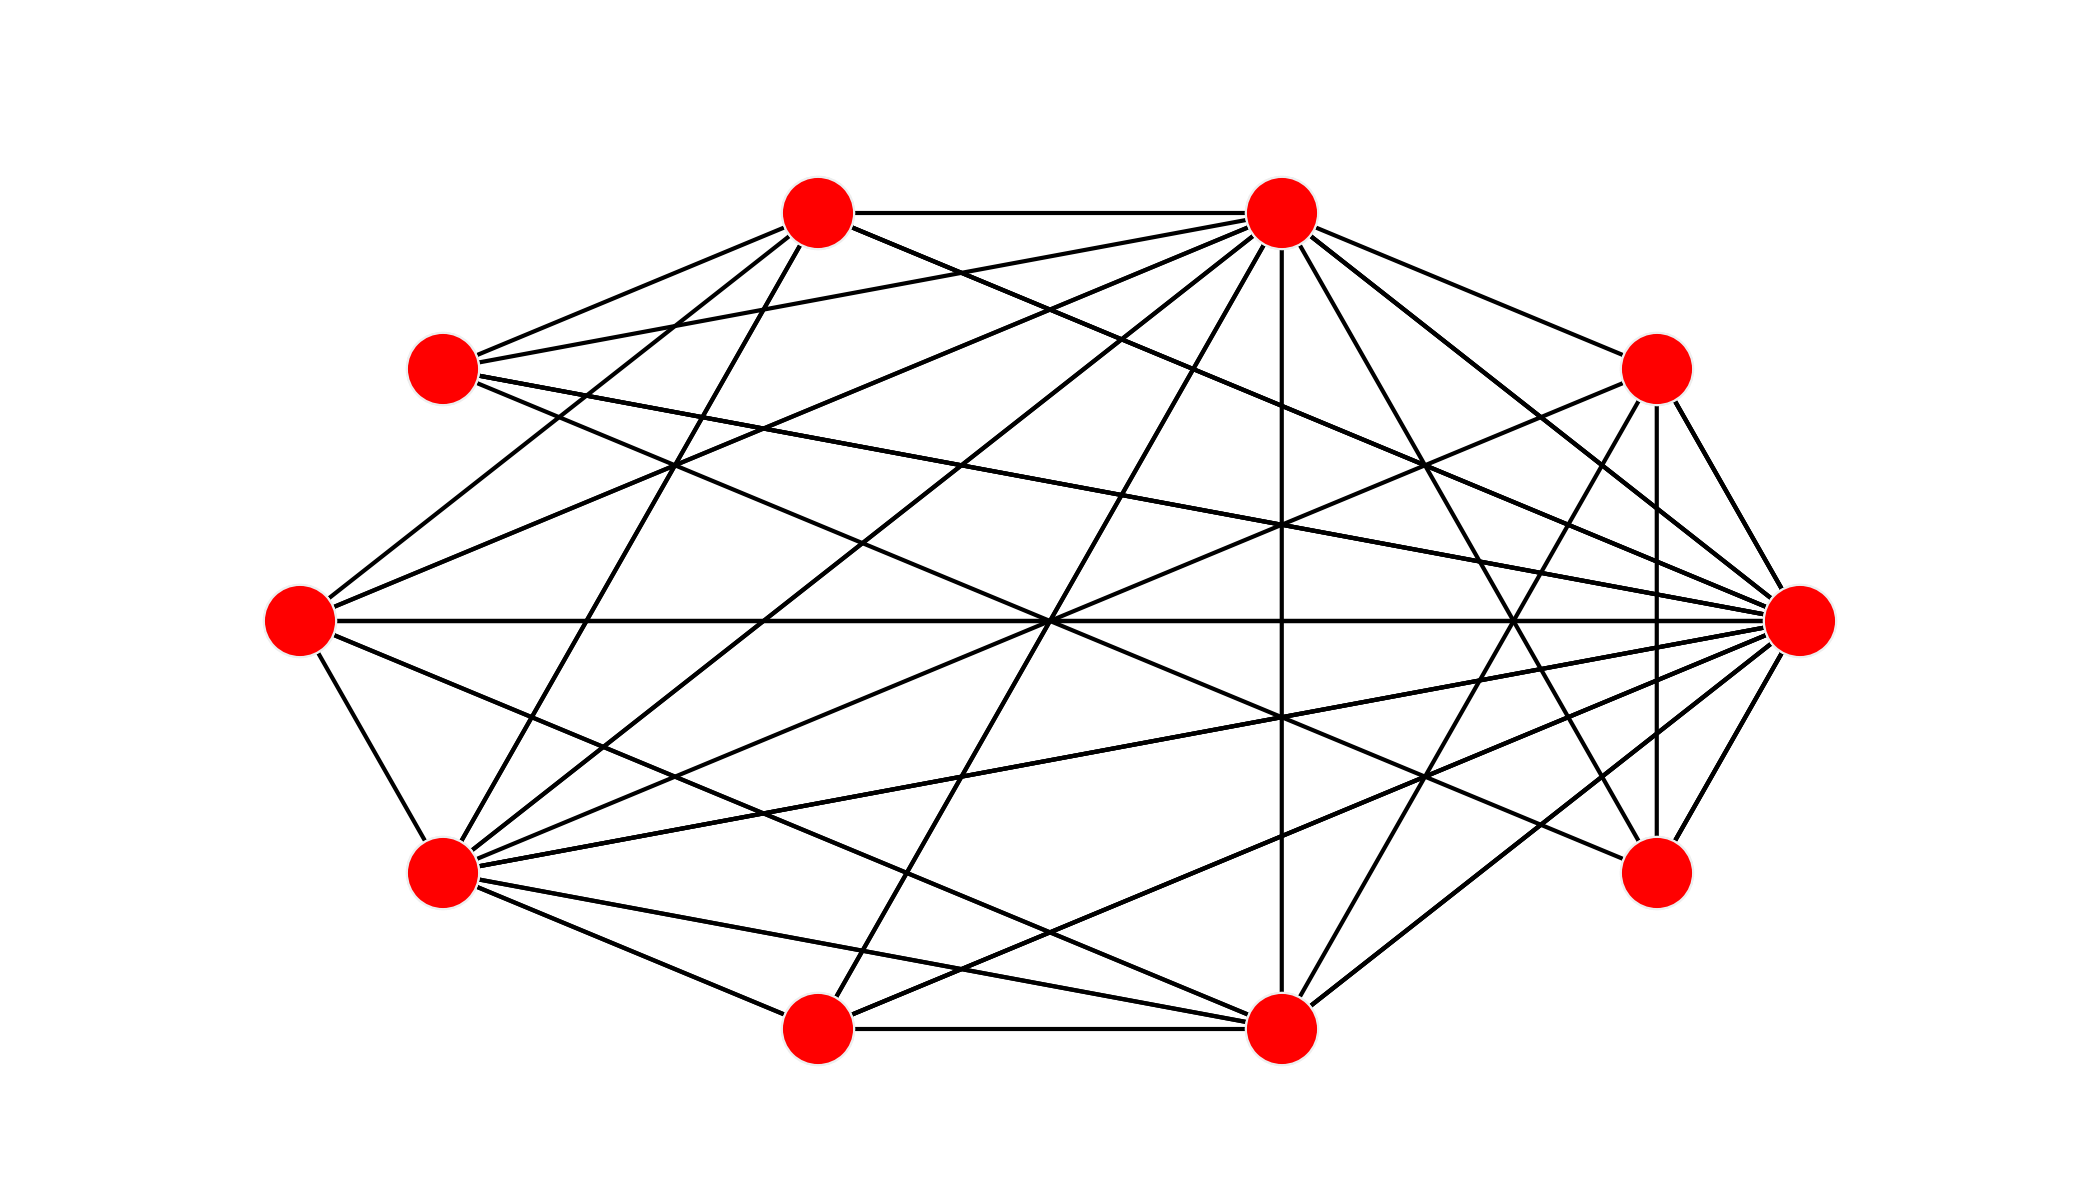
\includegraphics[width=1.2\linewidth]{graph_nonuniform_10_24} \\ в)}
  \end{minipage}
  \caption{Примеры графов, неоднородных по степеням вершин. \\ Слева направо: 12, 18, 24 ребра, во всех случаях 10 вершин, а 5 ребер ---~случайны.}
  \label{img:graphs-nonuniform}  
\end{figure}

Эксперимент состоит в том, чтобы при фиксированном числе ребер для трех групп графов~--- сильно однородных, сильно неоднородных и случайных ~--- измерить скорость сходимости модели. 

Две серии результатов приведены ниже:

\begin{figure}[H]
\begin{minipage}[h]{0.45\linewidth}
    \center{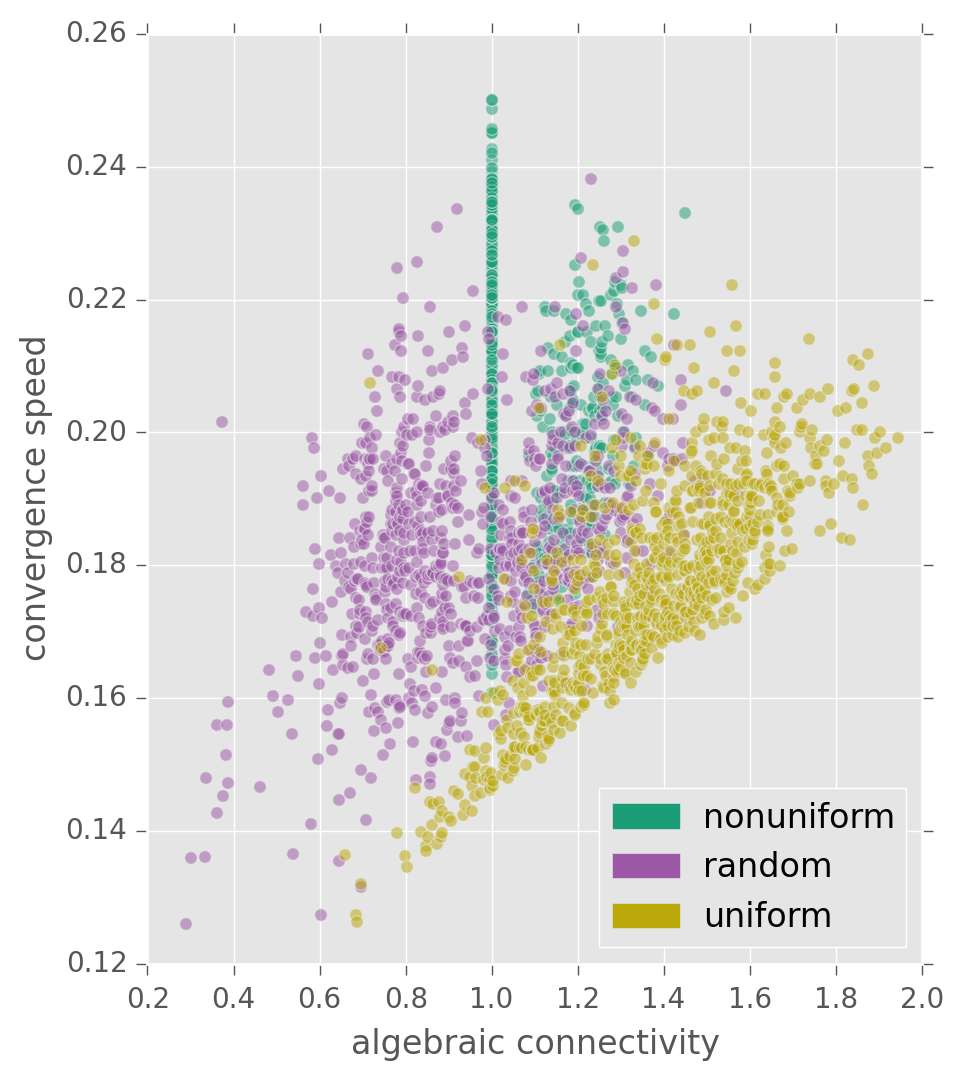
\includegraphics[width=1.0\linewidth]{convergence_speed_graph_comparison_15_30} \\ а)}
  \end{minipage}
  \hfill
  \begin{minipage}[h]{0.45\linewidth}
    \center{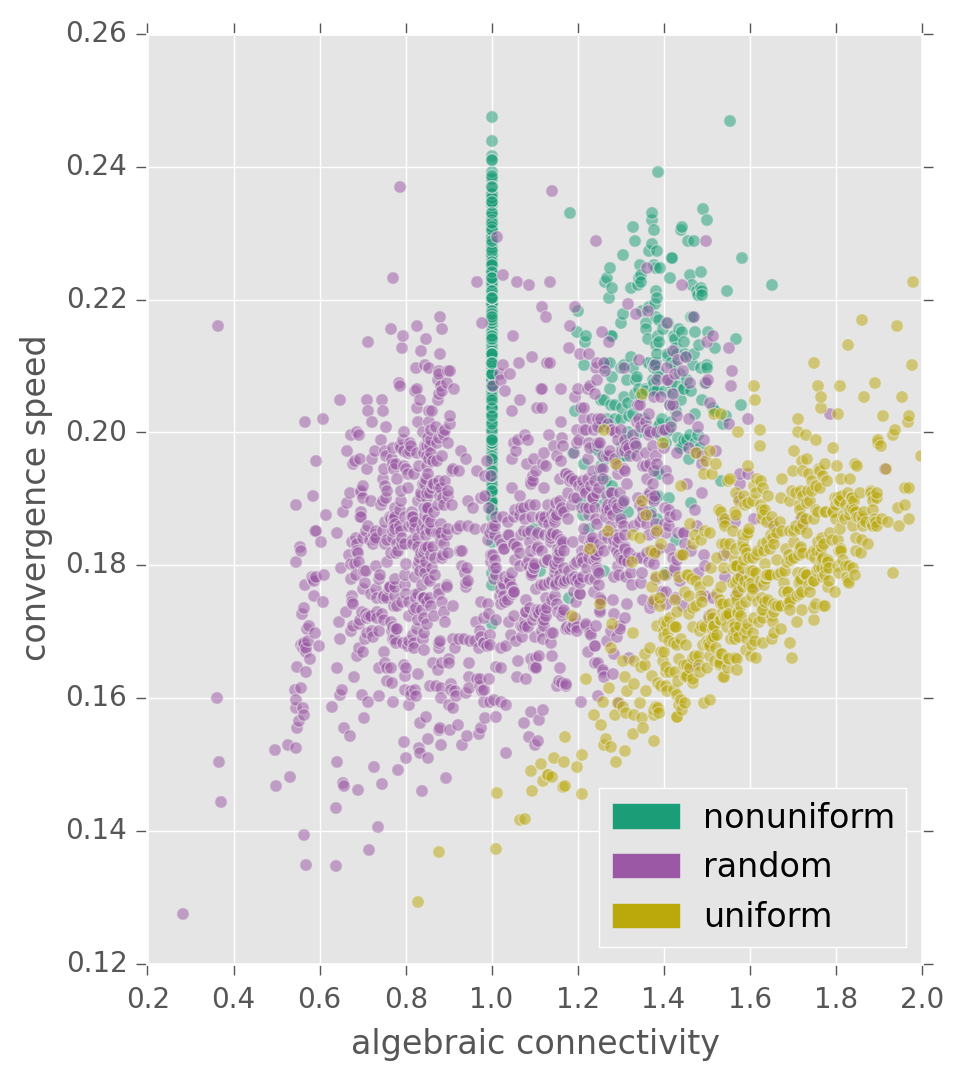
\includegraphics[width=1.0\linewidth]{convergence_speed_graph_comparison_21_50} \\ а)}
  \end{minipage}
  \caption{Скорость сходимости и алгебраическая связность при фиксированном числе ребер для трех групп графов: неоднородные графы (зеленый), однородные (желтый) и случайные графы (фиолетовый). В случае~а)~15 вершин и 30 ребер; в случае~б)~21 вершина и 50 ребер.}
    \label{img:graphs-comparison-1}  
\end{figure}

Ниже представлены данные для всех возможных чисел ребер на одном графике:


\begin{figure}[H]
    \center{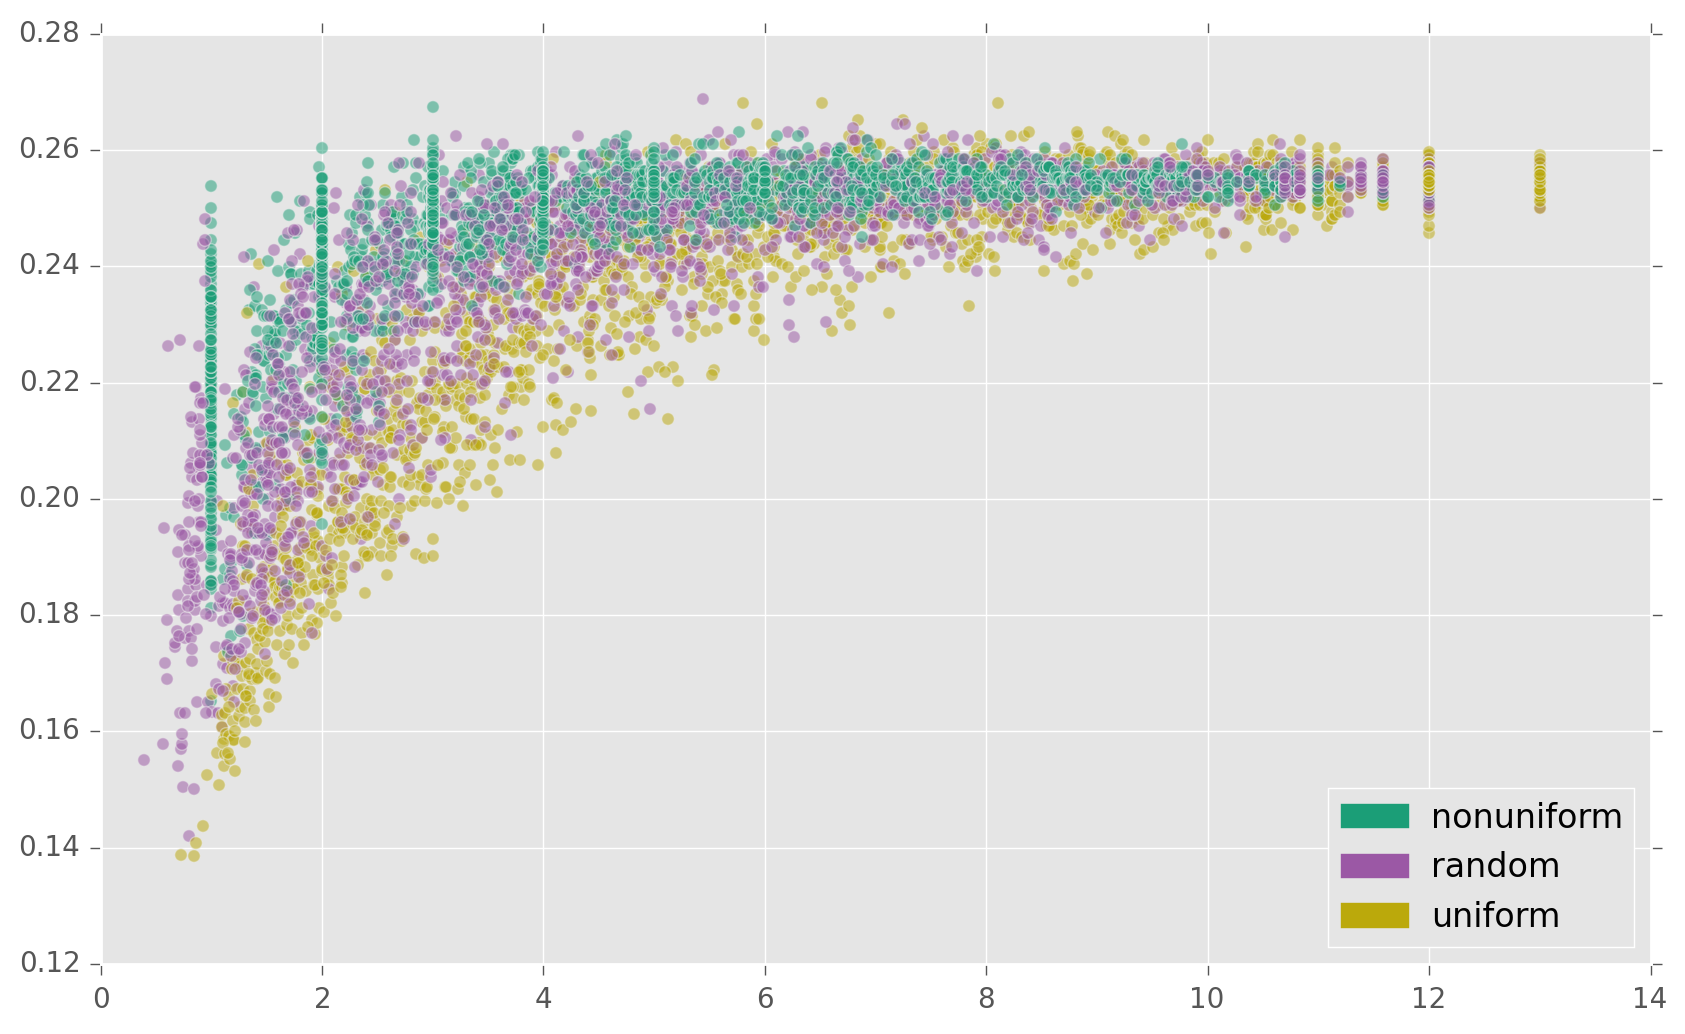
\includegraphics[width=0.9\linewidth]{convergence_speed_graph_comparison} 
  \caption{Скорость сходимости для трех групп графов: неоднородные графы (зеленый), однородные (желтый) и случайные графы (фиолетовый). Количество вершин равно 15.}
    \label{img:graphs-comparison}  
\end{figure}


\clearpage
